%*******************************************************************************
%***************************** Cellular Automata Chapter ***********************
%*******************************************************************************
\chapter{Cellular Automata}
\label{ch:CA}
\dictum[Richard Feynman]{There are many interesting phenomena … which involve a mixture of physical phenomena and physiological processes, and the full appreciation of natural phenomena, as we see them, must go beyond physics in the usual sense. We make no apologies for making these excursions into other fields, because the separation of fields, as we have emphasized, is merely a human convenience, and an unnatural thing. Nature is not interested in our separations, and many of the interesting phenomena bridge the gaps between fields.}%
\vskip 1em

%\section{Introduction}\label{cellularAutomataIntroduction}
\lettrine[lines=3,lhang=0.33,lraise=0,loversize=0.15]{N}{owadays} most of the basic natural phenomena are well described and known, thanks to the effort of lots of scientist that studied the basic physic's laws for centuries; for example, the freezing of water or the conduction that are well know and qualitative analyzed. Natural system are usually composed by many parts that interact in a complex net of causes/consequences that is at least very difficult but most of the times impossible to track and so to describe. Even if the single component are each very simple, extremely complex behavior emerge naturally due to the cooperative effect of many components. Much has been discovered about the nature of the components in natural systems, but little is known about the interactions that these components have in order to give the overall complexity observed.
Classical theoretical investigations of physical system have been based on
mathematical models, like differential equations, that use calculus as tool
to solve them, which are able to describe and allow to understand the
phenomena, in particular for those that can be described by which are linear
differential equation\footnote{Some electro-magnetism phenomena, for instance,
can be described by linear differential equations.} that are easy solvable with calculus.
Problems arise when non-linear differential equations come out from the
modellation of the phenomena, like fluid turbulence\footnote{Conventionally
described by Navier-Strokes differential equation.}.
Classical approach usually fails to handle these kind of equations due to the
too high number of components, that make the problem intractable even for a computer based numerical approach.
Another approach to describe such systems is to distill only the fundamental and
essential mathematical mechanism that yield to the complex behavior and at  the
same time capture the essence of each component process. Cellular automata are a
\begin{figure}
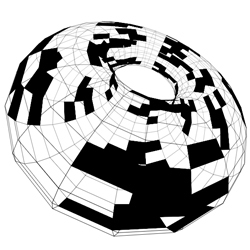
\includegraphics[scale=0.8]{./images/CA_FDM/torus-2}
\caption{3D cellular automata with toroidal cellular space.}\label{torus}
\end{figure}

candidate class of such systems and are well suitable for the modellation and
simulation of a wide class of systems, in particular those ones constructed from
\textbf{many identical} components, each (ideally) simple, but together capable
of complex behaviour\cite{Toffoli1984}\cite{toffoli1987}. In literature there
are lots applications of cellular automata in a wide rage of class problems from
gas\cite{Frisch1986} and fluid turbulence\cite{Succi1991} simulation to
macroscopic phenomena\cite{Gregorio1999} like epidemic
spread\cite{Sirakoulis2000}, snowflakes and lava
flow\cite{Crisci2004}\cite{Spataro2010}.
CA were first investigated by S. Ulam working on growth of crystals using
lattice network and at the same time by Von Neumann in order to study
self-reproduction\cite{Neumann1966}; it was not very popular until the 1970 and
the famous Conway's game of life\cite{conway1970}, then was widely studied on
the theoretical viewpoint, computational universality were
proved\footnote{CA is capable of simulating a Turing machine, so, in theory is
capable of computing every computable problems(Church-Turing
thesis). Game of life, for example was proved to be capable
of simulating logical gates (with special patterns as
\textit{gliders} and \textit{guns})}\cite{Thatcher1970} and then mainly
utilised, after 1980's, as parallel model due to its intrinsically parallel nature implemented on parallel computers\cite{Margolus1986}.




\section{Informal Definition}

Informally a \emph{cellular automata} (CA) is a mathematical model that
consists of a discrete lattice of sites  and a value, the state, that is
updated in a sequence of discrete timestamps (steps) according to some logical rules that
depend on a neighbor  sites of the cell. Hence CA describe systems whose the
overall behavior and evolution of the system may be exclusively described on the basis of local
interactions\cite{wolfram1984}, property also called centrism.
The most stringent and typical characteristic of the CA-model is the restriction
that the local function does not depend on the time t or the place i: a cellular automaton has homogeneous
space/time behavior. It is for this reason that ca are sometimes referred to as
\textit{shift-dynamical} or \textit{translation invariant} systems. From another
point of view we can say that in each lattice site resides a finite state
automaton\footnote{A simple and well know computational model. It has inputs,
outputs and a finite number of states (hence a finite amount of memory);
An automata changes state at regular time-steps.}  that take as
input only the states of the cells in its neighborhood (see figure \ref{amod3Automata}).

\subsection{Cellular space dimension and geometry}
The cellular space is a \emph{discrete} d-dimensional lattice of sites (see
figure \ref{spazioCellulare}).
For 1-D automaton the only way to discretize the space is in a one-dimensional
grid. For automaton with dimensionality higher than 1 the shape of each cell can
be different than squared. In 2D tessellation for example each cell can be
hexagonal or triangular instead of squared. Each tessellation present advantages
and disadvantages. For instance the squared one does not give any graphical
representation problem\footnote{Each cell could be easily mapped onto a
pixel.}, but present problems of anisotropy for some kind of
simulations\footnote{The HPP model for fluid simulation was highly anisotropyc due to the squared tessellation.}\cite{Frisch1986}.
An Hexagonal tessellation can solve the anisotropy problem\cite{wolfram1986} but
presents obvious graphical issues. Often, to avoid complications
due to a boundary, periodic boundary conditions are used, so that a two-dimensional grid
is the surface of a torus (see picture \ref{torus}).


\subsection{Neighborhood}
\begin{figure}
\centering
\caption{Examples of cellular spaces. (a) 1-D, (b) 2-D squared cells,
(c) 2-D hexagonal cells, (d) 3-D cubic cells.}\label{spazioCellulare}
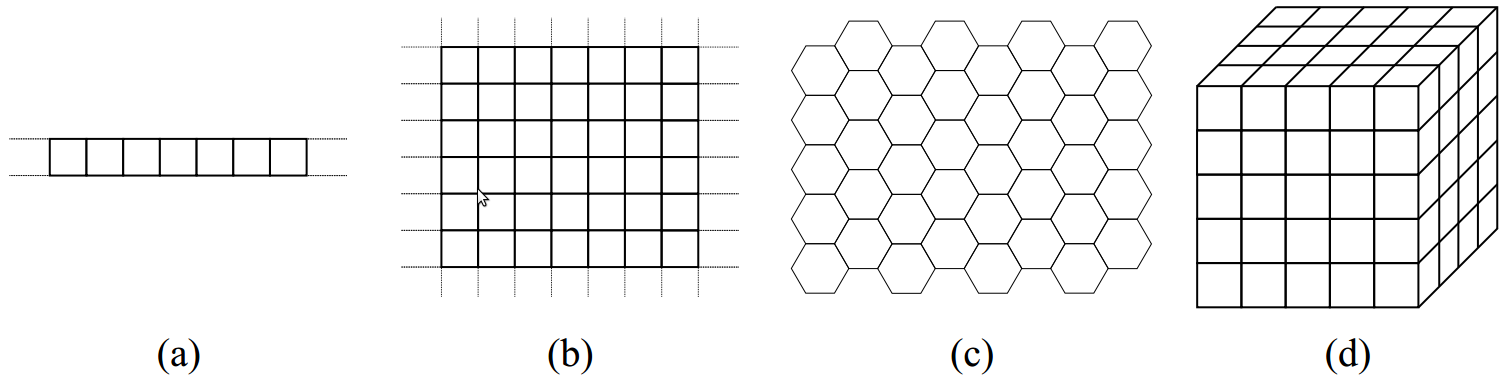
\includegraphics[scale=0.23]{./images/CA_FDM/spazioCellulare}
\end{figure}
The evolution of a cell's state is function of the states of the neighborhood's
cells. The geometry and the number of cells that are part of the neighborhood
depends on the tessellation type, but it has to have three fundamental
properties:
\begin{enumerate}
  \item \textbf{Locality}. It should involve only a 'limited' number of cells.
  \item \textbf{Invariance}. It should not be changed during the evolution.
  \item \textbf{Homogeneity}. It has to be the same for each cell of the
  automaton.
\end{enumerate}
Typically neighborhood ``surrounds'' the central cell. For 1-D cellular automata
its borders are identified with a number \begin{math}r \end{math} called
\textit{radius}\cite{wolfram1983}. A \begin{math}r=2\end{math} identify
\begin{math}n=2r+1\end{math} cells in a 1D lattice: the central cell plus the
right and left cells. Typical 2D cellular space neighborhood are the those of
Moore and von Neumann neighborhood. The number of cells in the Moore
neighborhood of range r is the odd squares \begin{math}(2r+1)^2,\end{math} the
first few of which are 1, 9, 25, 49, 81, and so on as r is increased.
Von Neumann's one consist of the central cell plus the cell at north, south,
east, and west of the central cell itself. Moore's (\begin{math}r=1\end{math})
one add  the farther cells at north-east, south-east, south-west and north-west
(see figure \ref{mooreNeigh}).



\begin{figure}
\centering
\caption{Examples of different kind of neighborhood with
different radius values.}\label{mooreNeigh}
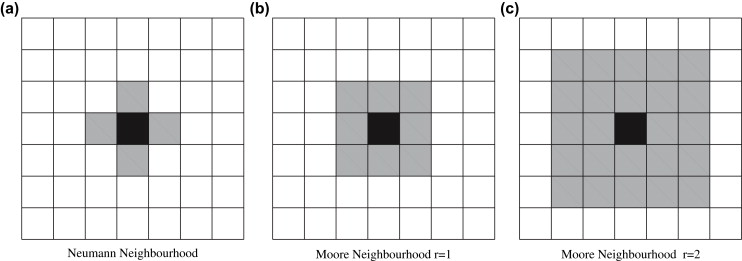
\includegraphics[width=1.0\textwidth]{./images/CA_FDM/mooreNeigh}
\end{figure}

\subsection{Transition Function}
The evolution of the cell's state is decided by the transition function that
is applied at the same time and on each cell. Usually that transition function
is deterministic and defined by a \textit{look-up} table only when the total
number of state for each cell is small\footnote{Otherwise the dimension of that table would be enormous because the number of entries is exponential in the number of
states.} otherwise is defined by an algorithmic procedure.
It may be probabilistic, in the case of stochastic cellular automata.

\section{Formal Definition}
Cellular automata are dynamic models that are
discrete in time, space and state. A simple cellular
automaton A is defined by a lattice of cells each containing a finite state
automaton so we briefly give its definition.

\subsection{Finite State Automaton}\label{DFA}
Also known as deterministic finite automata (DFAs) or as deterministic finite
state machines, are ones of the most studied and simple computational model
known.
 It is a theoretical model of computation\footnote{Language recognition
problem solvers.} that can be in a finite number of states, only one at a time,
the current state. Its state can change in response of inputs taken by a
transition function that describe the state change given the current state and
\begin{table}
\scalebox{1.2}{
\begin{tabular}{|c|ccccc|}\hline
\(\delta\) & \(a\) & \(b\) & \(c\) & \(d\) & \(e\) \\ \hline
\(q_0\) &\(q_0\) &\(q_0\) &\(q_2\) &\(q_1\) &\(q_1\)\\  
\(q_1\) &\(q_1\) &\(q_3\) &\(q_1\) &\(q_1\) &\(q_1\)\\  
\(q_2\) &\(q_3\) &\(q_2\) &\(q_2\) &\(q_0\) &\(q_1\)\\  
\(q_3\) &\(q_0\) &\(q_1\) &\(q_1\) &\(q_0\) &\(q_1\) \\ 
\hline 
 \end{tabular}
}
 \caption{Tabular representation of a DFM's next-state function}
 \label{tab:tabularTransitionFunction}
\end{table} 
the received input of the automata.
Its a much more restrictive in its capabilities than a Turing
machines,\footnote{For example we can show that is not possible for an
automaton to determine whether the input consist of a prime number of symbols.}
but they are still capable to solve simpler problems, and hence to recognize
simpler languages, like well parenthesized string; More in general they are capable
to recognize the so called \emph{Regular languages}\footnote{Languages
defined by regular expressions and generated by regular grammar, Class 3 in
Chomsky classification. We can prove that for each language L accepted by a DFA
exists a grammar \begin{math}L_G \end{math} s.t. \begin{math} L=L_G\end{math}},
but they fail for example in parsing \emph{context-free} languages.
More formally a DFA is a 5-tuple:
\[M = <Q,\Sigma,\delta,q_0,F>\] 

\begin{itemize}
  \item \textit{Q} is a finite, nonempty, set of states.
\item \begin{math}\Sigma\end{math} is the alphabet
\item \begin{math} \delta : Q \times \Sigma \longmapsto Q  \end{math} is the
transition function (also called next-state function, may be represented in
tabular form  (see table
\ref{tab:tabularTransitionFunction})
\item \begin{math}q_0 \end{math} is the initial (or starting) state :
\begin{math} q_0 \in  Q \end{math}
\item  \begin{math}F \end{math} is the set, possibly empty, of final states :
\begin{math} F \subseteq Q \end{math}

\end{itemize}



A run of DFA on a input string \begin{math}u = a_0,a_1,\ldots,a_n\end{math} is a
sequence of states \\ \begin{math} q_0,q_1,\ldots,q_n\end{math} s.t.
\begin{math}q_i  \overset{a_i}{\longmapsto} q_{i+1} \end{math},
\begin{math} 0 \leq i \le n\end{math}. It means that for each couple of state
and input the transition function deterministically return the next DFA's
state \\ \begin{math}q_i=\delta(q_{i-1},a_{i}) \end{math}.
For a given word \begin{math}\textit{w}\in \Sigma^* \end{math} the DFA has a
unique run (it is deterministic), and we say that it \textbf{accepts} w if the
last state \begin{math}q_n \in F \end{math}. A DFA recognizes the
language L(M) consisting of all accepted strings.


Figure \ref{amod3Automata} is an example of DFA\footnote{Graph representation
is the most common way to define and design DFA. Nodes are the states, and
the labelled edges are the possible states transition from a state \textit{u}
to a state \textit{w} given a certain input.
Note that, because the automaton is deterministic is not possible for two
edges to point to two different nodes if same labelled.}.
It accepts the language made up of strings with a number N s.t \begin{math}N
\;mod\; 3 = 0 \end{math}
\begin{itemize}
  \item\begin{math} \Sigma = \{a,b\}\end{math}
  \item \begin{math} Q = \{t_0,t_1,t_2\}\end{math}
  \item \begin{math} q_0 = t_0\end{math}
  \item \begin{math} F = \{t_0\} \end{math}
\end{itemize}


If we execute the DFA on an input string S=\{aaabba\} we can see that at time
t=0 the DFA is in the initial state \begin{math}t_0\end{math} and the first
symbol of S is read.
The transition function is applied once per each symbol is S
(i.e. \begin{math}\left\vert{S}\right\vert\end{math}). The only rule that match 
the current state and input is \begin{math}\delta=(t_0,a)=t_1 \end{math} hence the
new state is \begin{math}t_1\end{math}. The DFA accept the string only if  there
is not any input left and the current state is the final state
\begin{math}q_f\end{math}\footnote{Previously we stated that F was a set but
we can assume that there is only one final state
(\begin{math}\left\vert{F}\right\vert=1\end{math}), because it is easy prove
that exist a DFA with only one final state given a generic DFA
(\begin{math}\left\vert{F}\right\vert \geq 1\end{math}). We add one more state
\begin{math}q_f\end{math} and for each final state \begin{math}q_i \in
F\end{math} we define new rules of the type \begin{math}\delta(q_i,*)=q_f, * \in I \end{math}.}.
S is not accepted by the DFA defined in the example \ref{amod3Automata} because
at the end of the computation the reached state is \begin{math}t_1\end{math}
that is not a final state.
 \[
 t_0\overset{\delta(t_0,a)}
 {\longmapsto}t_{1}\overset{\delta(t_1,a)}
 {\longmapsto}t_{2}\overset{\delta(t_2,a)}
 {\longmapsto} t_{0}\overset{\delta(t_0,b)}
 {\longmapsto}t_{0}\overset{\delta(t_0,b)}
 {\longmapsto}t_{0}\overset{\delta(t_0,a)}
 {\longmapsto} t_{1}
\]
On the input \begin{math}S^1=\{abababb\}\end{math} the DFA accept:
 \[
 t_0\overset{\delta(t_0,a)}
 {\longmapsto}t_{1}\overset{\delta(t_1,b)}
 {\longmapsto}t_{1}\overset{\delta(t_1,a)}
 {\longmapsto} t_{2}\overset{\delta(t_2,b)}
 {\longmapsto}t_{2}\overset{\delta(t_2,a)}
 {\longmapsto}t_{0}\overset{\delta(t_0,b)}
 {\longmapsto}t_{0}\overset{\delta(t_0,b)}
 {\longmapsto}\mathbf{t_{0}}
\]
\begin{figure}
\begin{center}
  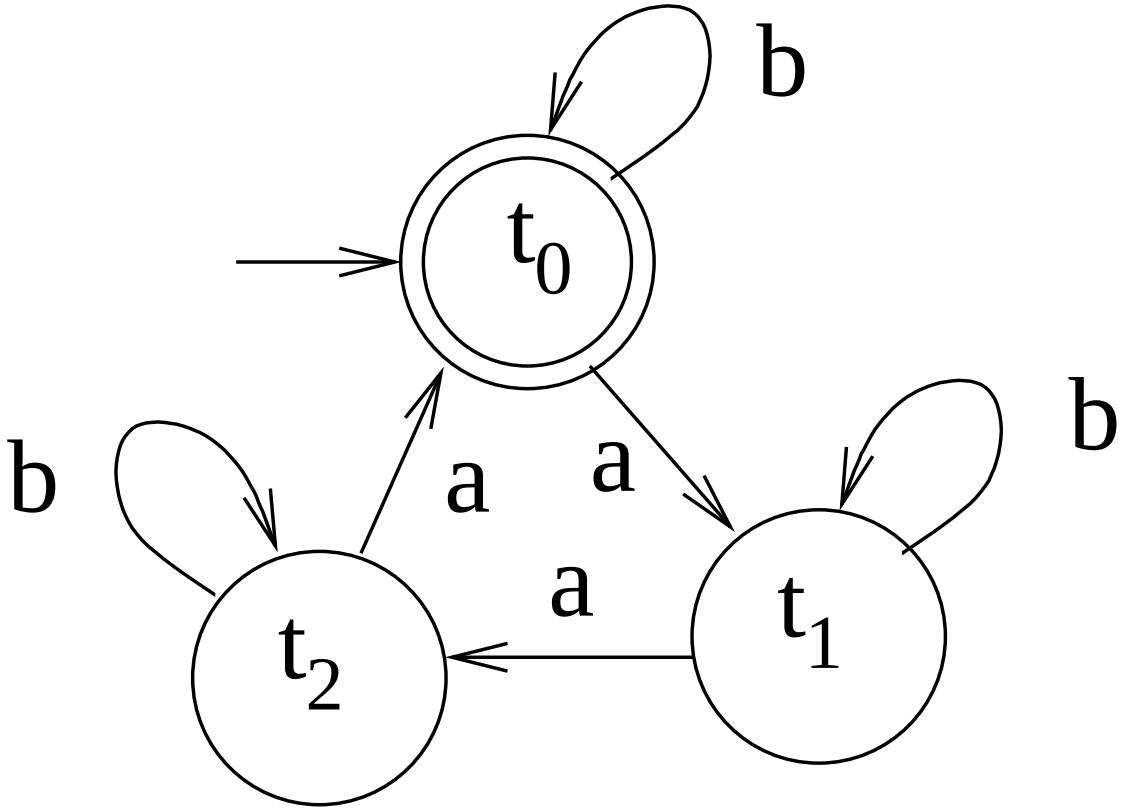
\includegraphics[scale=0.17]{./images/CA_FDM/amod3Automata}
  \caption{Graph representation of a DFA}
  \label{amod3Automata}
\end{center}
\end{figure}



\section{Homogeneous Cellular Automata}\label{homogeneousCellularAutomata}
Formally a CA \emph{A} is a quadruple \begin{math} A=<Z^d,X,Q,\sigma>\end{math}
where:
\begin{itemize}
  \item \begin{math}\mathbb{Z}^d=\{i=(i_1,i_1,\ldots,i_d)\mid i_k \in
  \mathbb{Z}, \forall k=1,2,\ldots,d \}\end{math} is the set of cells of the d-dimensional
   Euclidean space.
  \item \begin{math}X\end{math} is the neighborhood, or neighborhood template; a
  set of m d-dimensional vectors (one for each neighbor)
  \[\xi_j=\{\xi_{j1},\xi_{j2},\ldots,\xi_{jd}\} \;,\: 1\leq j \leq m\] that
  defines the set of the neighbors cells of a generic cell
  \begin{math}i=(i_1,i_1,\ldots,i_d)\end{math}
  \[
  N(X,i)=\{i+\xi_0,i+\xi_2,\ldots,i+\xi_d\}
  \] where \begin{math}\xi_0\end{math} is the null vector. It means that the
  cell \begin{math}i\end{math} is always in its neighborhood and we refer to it
  cell as \emph{central cell}  (see example below).
\item Q is the finite set of states of the elementary automaton EA.
  
  \item \begin{math}\sigma=Q^m \rightarrow Q \end{math} is the transition
  function of the EA. \begin{math}\sigma\end{math} must specify
  \begin{math}q_k \in Q \end{math} as successor  state of the central cell.
  If there are \begin{math}m\end{math} cells in the neighborhood of the central
  cell including itself, then there are
  \begin{math}{\left\vert{Q}\right\vert}^m\end{math} possible neighborhood's
  state configuration. It  means that there are
  \begin{math}{\left\vert{Q}\right\vert}^{{\left\vert{Q}\right\vert}^m}\end{math}
  possible transition functions. Plus we can see that the tabular definition of
  the next-state function is unsuitable for practical purpose. It should have
  \begin{math}\left\vert{\sigma}\right\vert={\left\vert{Q}\right\vert}^m\end{math}
  entries, an exceedingly large number.
  \item \begin{math}\tau=C \longrightarrow C \longmapsto
  \sigma(c(N(X,i))) \end{math} where 
  where $C=\{c \colon Z^d
  \rightarrow Q\}$
  is called the set of the possible configuration and 
  \begin{math}
  C(N(X,i)))\end{math} is the set of states of the neighborhood of \textit{i}.
\end{itemize}



For example consider a 2D cellular automata with Moore neighborhood and a
generic cell c=(10,10) and \begin{math}{\left\vert{Q}\right\vert}=5\end{math}
possible state for each cell .
\[X=\{\xi_{0},\xi_{1},\xi_{2},\xi_{3},\xi_{4},\xi_{5},\xi_{6},\xi_{7},\xi_{8}\}
=\]\[=\{(0,0),(-1,0),(0,-1),(1,0),(0,1),(-1,-1),(1,-1),(1,1),(-1,1)\}
\]
Hence the set of the cells belonging to the neighborhood(defined by X) of
c=(10,10) is:
\begin{math}V(X,c)=\{(0,0)+c,(-1,0)+c,(0,-1)+c,(1,0)+c,(0,1)+c,(-1,-1)+c,(1,-1)+c,(1,1)+c,(-1,1)+c\}
\end{math} 
\[=\{(10,10),(9,10),(10,9),(11,10),(10,11),(9,9),(11,9),(11,11),(9,11)\}
\]
and the total number of entries for the tabular definition of the
transition-function is  \begin{math}{\left\vert{Q}\right\vert}^{\left\vert{X}\right\vert}=
5^9=1953125\end{math} and the total number of possible transition functions
is
\begin{math}{\left\vert{Q}\right\vert}^{{\left\vert{Q}\right\vert}^{\left\vert{X}\right\vert}}=
5^{5^9}=5^{1953125}\end{math}.



\section{Theories and studies}

\subsection{Elementary cellular automata}
The most simple AC we can imagine are the elementary cellular
automata\cite{wolfram1983}. They are one-dimensional periodic N cells array
\begin{math}\{C_i \mid 1\leq i \leq N, C_i \in \{0,1\} \}\end{math} each
with 2 possible state (0,1), and rules that depend only on nearest neighbor
value hence a radius r=1 neighborhood with a total number of involved cell
\begin{math}2r+1=2\times1+1=3\end{math} (central, right and left cells).
Since there are only \begin{math}2\times2\times2\times=2^{2r+1}=2^3=8\end{math} possible states for
the neighborhood of a given cell there are a total of
\begin{math}2^{2^3}=2^8=256\end{math} possible elementary automata (each of
which may be identified with a 8-bit binary number\cite{wolfram2002}).

\subsubsection{Wolfram's code}
The transition function  is \begin{math}F(C_{i-1},C_i,C_{i+1})\end{math} is
defined by a look-up table of the form stated in table
\ref{wolframcodeGeneral}, and an example of an instance of a function is given
(rule 110, an important rule on which \cite{cook2004} proved universal
computational power, as Wolfram had conjectured in 1985, and is arguably the
simplest Turing complete system\cite{wolfram2002}) in table
\ref{wolframcodeGeneral}.

\begin{table}
\caption{Encoding of a transition function for a generic elementary CA. On the
right the instance 110.}
\centering
\begin{tabular}{l}
\label{wolframcodeGeneral}

\hfill \\
\hline
  \begin{math}F(1,1,1)=\{0,1\}\end{math}  \\
  \begin{math}F(1,1,0)=\{0,1\}\end{math}  \\
  \begin{math}F(1,0,1)=\{0,1\}\end{math}  \\
  \begin{math}F(1,0,0)=\{0,1\}\end{math}  \\
  \begin{math}F(0,1,1)=\{0,1\}\end{math}  \\
  \begin{math}F(0,1,0)=\{0,1\}\end{math}  \\
  \begin{math}F(0,0,1)=\{0,1\}\end{math}  \\
  \begin{math}F(0,0,0)=\{0,1\}\end{math}  \\
\hline
\end{tabular}
\quad
\begin{math}\overset{instance}{\longrightarrow}\end{math}
\begin{tabular}{l}

\label{wolframcoderule}
\hfill \\
\hline
  \begin{math}F(1,1,1)=0\end{math}  \\
  \begin{math}F(1,1,0)=1\end{math}  \\
  \begin{math}F(1,0,1)=1\end{math}  \\
  \begin{math}F(1,0,0)=0\end{math}  \\
  \begin{math}F(0,1,1)=1\end{math}  \\
  \begin{math}F(0,1,0)=1\end{math}  \\
  \begin{math}F(0,0,1)=1\end{math}  \\
  \begin{math}F(0,0,0)=0\end{math}  \\
\hline
\end{tabular}
\end{table}

More generally Wolfram's code\cite{wolfram1983,wolfram2002} can be calculated 
Conventionally neighborhoods are sorted in non-decreasing order
,(111=7),(110=6),(101=5) etc., and the may be interpreted as a 8-digit number
\[01101110=2^0\times0+2^1\times1+2^2\times1+2^\times1+2^4\times0+2^5\times1+2^6\times1+2^7\times0=110\]


\begin{enumerate}
  \item List and sort in decreasing numerical (if interpreted as number) order
  all the possible configuration of the neighborhood of a given cell.
  \item For each configuration, list the state which the given cell will have,
  according to this rule, on the next iteration.
  \item Interprets the resulting list as binary number and convert it to
  decimal. That  is the Wolfram's code.
\end{enumerate}

Note that is not possible to understand from that code which is the size or the
shape of the neighborhood. Is tacit to suppose that those information are
already known.


\subsection{Wolfram's classification}
Mathematical analysis of CA may be not so straightforward despite their simple
definition. A first attempt to classify CA was attempted by
Wolfram\cite{wolfram2002}. He proposed a set of four classes for CA
classification that are the most popular method of CA classification, but they
suffer from a degree of subjectivity. Classification is based only on visual
valuations, that are obviously subjective. A more rigorous definition of these
classes is given in \footnote{They prove that decide the class(from the
wolfram's four one) of membership of a generic CA is an undecidable problem. Is
not possible to design an algorithm that solve this problem.}\cite{culik1998}.
Here the four Wolfram's classes.
\begin{enumerate}
  
  \item these CA have the simplest behavior; almost all initial conditions
  result in the same uniform initial state (homogeneous state).
  \item different initial conditions yield different final patterns, but
  these different patterns consist of an arrangement of a certain set of
  structures, which stays the same forever or repeats itself within a few
  steps(periodic structures).
  \item behavior is more complicated and appears random, but some repeated
  patterns are usually present (often in the form of triangles)(chaotic pattern).
  \item in some respects these are the most complicated class; these behave
  in a manner somewhere in between Class II and III, exhibiting sections
  both of predictable patterns and of randomness in their pattern
  formation(complex structures).
\end{enumerate}
He observed that the behavior of a meaningful class of Cellular Automata
by performing computer simulations of the evolution of the automata starting
from random configurations. Wolfram suggested that the different behavior of
automata in his classes seems to be related to the presence of different types
of attractors.In figures \ref{class12} and \ref{class34} some elementary automata divided in their classes.\footnote{Images courtesy of
\url{http://plato.stanford.edu/entries/cellular-automata/}}
 \begin{figure}
 \caption{Class 1 (a,b) and 2 (c,d) elementary cellular automata}
 \label{class12}
\centering
    \begin{subfigure}[b]{0.275\textwidth}
		\centering
		\label{fig:first}
		
		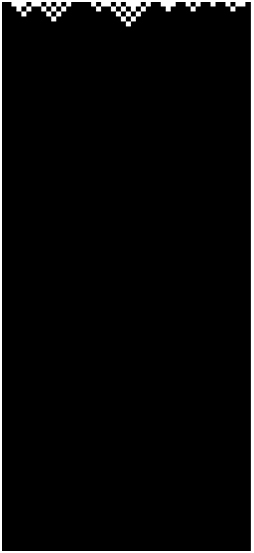
\includegraphics[scale=0.32]{./images/CA_FDM/rule250}
\caption[]{}%
   \end{subfigure}%
    \begin{subfigure}[b]{0.275\textwidth}
		\centering
		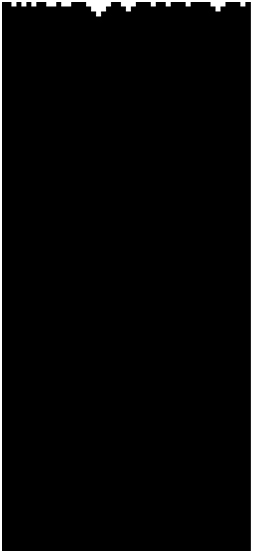
\includegraphics[scale=0.32]{./images/CA_FDM/rule254}
		\caption[]{}%
   \end{subfigure}%
   \hfill
       \begin{subfigure}[b]{0.275\textwidth}
   	\centering
   	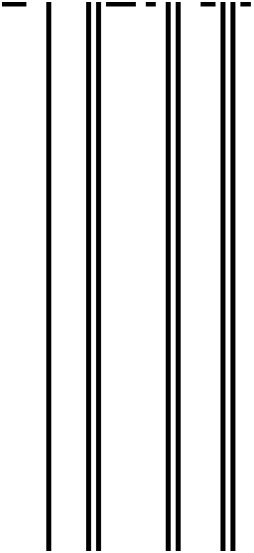
\includegraphics[scale=0.32]{./images/CA_FDM/rule4}
   	\caption[]{}%
   \end{subfigure}%
   \begin{subfigure}[b]{0.275\textwidth}
   	\centering
   	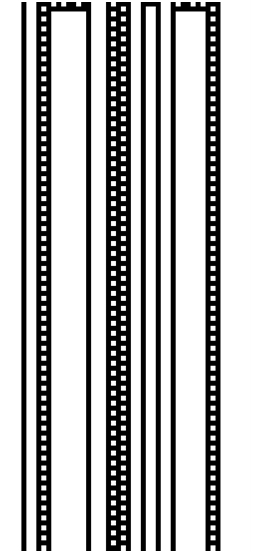
\includegraphics[scale=0.32]{./images/CA_FDM/rule108}
   \caption[]{}%
   \end{subfigure}%
        
\end{figure}

We can well see from these examples that automata from class 1 have all cells
ending up very quickly with the same value, in a homogeneous state and automata
from class 2 with a simple final periodic patterns.
Class 3 appear to be chaotic and non-periodic and automata from class 4 have
a mixed behaviour, complex-chaotic structures are locally propagated.
\subsection{At the edge of Chaos}
Class 4 automata are at \emph{the edge of chaos} and give a good metaphor for
the idea that the \textit{interesting} complexity (like the one exhibit by
biological entities and their interactions or analogous to the phase transition
between solid and fluid state of the matter, is in equilibrium between
stability and chaos\cite{Langton1990}.

\begin{quotation}
\em Perhaps the most exciting implication (of CA representation of biological
phenomena) is the possibility that life had its origin in the vicinity of a
phase transition and that evolution reflects the process by which life has
gained local control over a successively greater number of environmental
parameters affecting its ability to maintain itself at a critical balance point
between order and chaos.\\
(\textit{\textbf{Chris Langton} - Computation at the edge of chaos.
Phase transition and emergent computation - pag.13}).
\end{quotation}

 \begin{figure}
	\caption{Class 1 (a,b) and 2 (c,d) elementary cellular automata}
	\label{class12}
	\centering
	\begin{subfigure}[b]{0.275\textwidth}
		\centering
		\label{fig:first}
		
		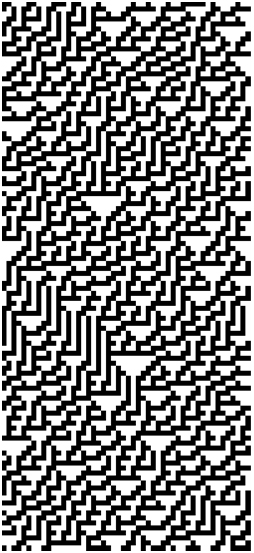
\includegraphics[scale=0.32]{./images/CA_FDM/rule30}
		\caption[]{}%
	\end{subfigure}%
	\begin{subfigure}[b]{0.275\textwidth}
		\centering
		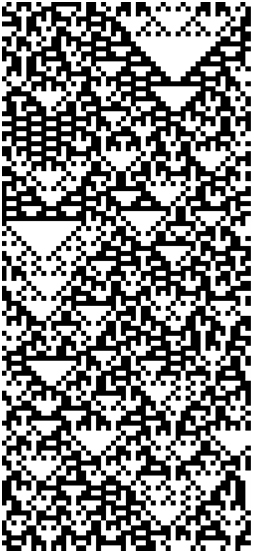
\includegraphics[scale=0.32]{./images/CA_FDM/rule90}
		\caption[]{}%
	\end{subfigure}%
	\hfill
	\begin{subfigure}[b]{0.275\textwidth}
		\centering
		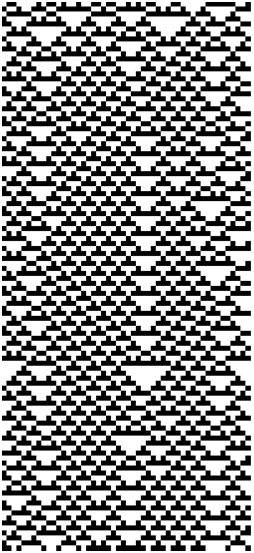
\includegraphics[scale=0.32]{./images/CA_FDM/rule54}
		\caption[]{}%
	\end{subfigure}%
	\begin{subfigure}[b]{0.275\textwidth}
		\centering
		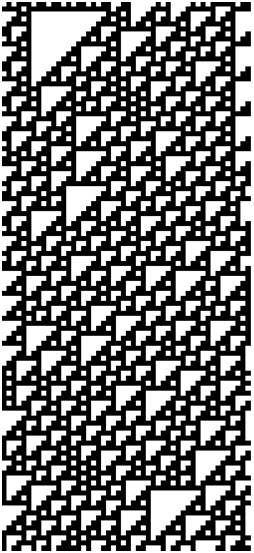
\includegraphics[scale=0.32]{./images/CA_FDM/rule110}
		\caption[]{}%
	\end{subfigure}%
	
\end{figure}



%%
% -------------- End of figure environment ----------------------%


Langton in his famous paper, \textit{Computation at the edge of chaos: phase
transition and emergent computation}\cite{Langton1990},was able to
identify, simply parametrizing the rule space, the various AC classes, the
relation between them and to ``couple'' them with the classical complexity classes.
He introduced the parameter \begin{math}\lambda\end{math}\cite{LangtonThesis1990}that, informally, is simply
the fraction of the entries in the transition rule table that are mapped  the
not-quiescent state.
\[\lambda=\frac{K^N-n_q}{K^N}\]
where:
\begin{itemize}
  \item K is the number of the cell states
  \item N the arity of the neighborhood
  \item \begin{math}n_q\end{math} the number of rules mapped to the quiescent
  state \begin{math}q_q\end{math}
\end{itemize}

\begin{figure}
\centering
\caption{Relation between lambda parameter and the CA
behaviors-Wolfram's classes.}\label{lambdaWolframClass}
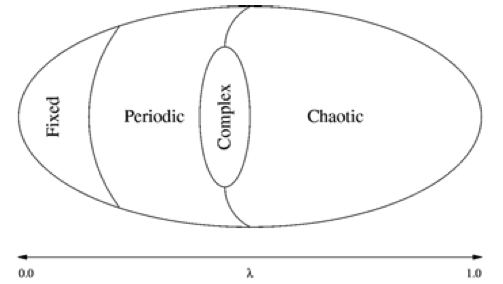
\includegraphics[scale=0.4]{./images/CA_FDM/edgeofchaos}
\end{figure}
Langton's major finding was that a simple measure such as it correlates with the
system behavior: as it goes from 0 to \begin{math} 1-\frac{1}{K}\end{math}(respectively the most
homogeneous and the most heterogeneous rules table scenario), the average
behavior of the system goes from freezing to periodic patterns to chaos and functions with an average 
value of \begin{math}\lambda\end{math} (see \cite{Langton1990} for a
more general discussion) are being on \emph{on the edge}(see figure \ref{lambdaWolframClass}).

He studied a entire family of totalistic CA with \begin{math}k=4
\end{math} and \begin{math}N=5\end{math} with \begin{math}\lambda\end{math}
varying in \begin{math}[0,0.75]\end{math}. He was able to determine that values
of \begin{math}\lambda\approx0.45\end{math} raise up to class 4 cellular
automata.
Computational system must to provide fundamental properties if it is
to support computation. Only CA  \emph{on the edge} show these properties on
manipulating and store information data.
Here the properties that a computational system as to provide:
\begin{description}
  \item[Storage] \hfill \\
  Storage is the ability of the system of preserving information for
arbitrarily long times
  \item[Transmission] \hfill \\
  Transmission is the propagation of the information in the
form of signals over arbitrarily long distance
  \item[Modification] \hfill \\
Stored and transmitted
information is the mutual possible modification of two signals.

\end{description}

Storage is coupled with less entropy of the system, but transmission and
modification are not. Few entropy is associated with CA of Class 1 and 2 and
high entropy with class 3. Class 4 is something in between, the cells cooperate
and are correlate each other, but not too much otherwise they would be overly
dependent with one mimicking the other supporting computation in all its aspects
and requirements. Moreover class 4 CA are very dependent from the initial
configuration opening to the possibility to encode programs in it.

\subsection{Game of life}
\label{sect:GOL}
CA are suitable for representing many physical, biological, social and other
human phenomena. But they are a good tool to study under which condition a
physical system supports the basic operation constituting the capacity to
support computation. Game of life is a famous 2D
cellular automaton of '70s early studied (and perhaps proved) for its universal
computation capacity.



\subsubsection{Game of life - brief definition} 
The Game of Life is totalistic CA\footnote{A totalistic cellular automaton is a cellular automata in which the rules depend only on the	total (or equivalently, the average) of the values of the cells in a neighborhood.} that can be thought as an infinite two-dimensional orthogonal grid of square cells, each of which is in one of two possible states, \emph{dead} or \emph{alive}. Every cell interacts with the eight adjacent neighbors belonging to the Moore neighborhood. At each time step, one of the following transitions occur:
	\begin{itemize}
	\item \emph{Birth}: If the cell is in the state \textbf{\textit{dead}} and
	the number of alive neighbors is \textbf{\textit{3}}, then the cell state
	becomes alive (1).
	\item \emph{Survival}: If the cell is in the state \textbf{\textit{alive}}
	and the number of alive neighbors is \textbf{\textit{2 or 3}}, then the cell
	state is still alive (1).
	\item \emph{Dead}: If the cell is in the state \textbf{\textit{alive}} and
	the number of alive neighbors is \textbf{\textit{less than 2 or higher
			than 3}}, then the cell state becomes dead (0).
\end{itemize}
The initial configuration of the system specifies the state (dead
or alive) of each cell in the cellular space. The evolution of the
system is thus obtained by applying the above rules (which define
the cell's transition function) simultaneously to every cell in
the cellular space, so that each new configuration depends on the
one at the current step. The rules continue to be applied
repeatedly to create further generations.

Formally the Game of Life CA can be defined as follows:
$$Life = < R, X, Q, \sigma >$$ where:
\begin{itemize}
	\item $R$ is the set of points, with integer coordinates, which
	defines a two-dimensional toroidal cellular space. The generic
	cell in $R$ is individuated by means of a couple of integer
	coordinates $(i, j)$, where $0 \leq i < i_{max}$ and $0 \leq j <
	j_{max}$. The first coordinate, $i$, represents the row, while
	the second, $j$, the column. The cell at coordinates $(0,0)$ is
	located at the top-left corner of the computational grid
	(cf. Figure \ref{fig:2Dneighborhood}b).
	
	\item $X = \{(0,0), (-1, 0), (0, -1), (0, 1), (1, 0), (-1,-1),
	(1,-1), (1,1), (-1,1)\}$ is the Moore neighborhood relation. The
	neighborhood coordinates of the generic cell of coordinate $(i,
	j)$ is given by
	$$N(X, (i, j)) = $$
	$$= \{(i, j)+(0,0), (i, j)+(-1, 0), \dots, (i, j)+(-1,1)\} =$$
	$$= \{(i, j), (i-1, j), \dots, (i-1,j+1)\}$$ Here, a subscript
	operator can be used to index cells belonging to the
	neighborhood. Let $|X|$ be the number of elements in X, and $n
	\in \mathbb{N}$, $0 \leq n < |X|$; the notation
	
	$$N(X, (i, j), n)$$
	
	represents the coordinates of the $n^{th}$ neighborhood of the
	cell $(i,j)$. Thereby, $N(X, (i, j), 0) = (i, j)$, i.e. the
	central cell, $N(X, (i, j), 1) = (i-1, j)$, i.e. the first
	neighbor, and so on (cf. Figure \ref{fig:2Dneighborhood}b).
	
	\item $Q = \{0, 1\}$ is the set of cell states, 0 representing the
	dead state, 1 the alive one.
	
	\item $\sigma : Q^9 \rightarrow Q$ is the deterministic cell
	transition function. It is composed by one elementary process,
	which implements the aforementioned transition rules.
\end{itemize}

The Game of Life is a class 4 Wolfram's taxonomy CA, because
\say{rich and complex structures, stable blocks and moving patterns come into existence even starting from a completely random configuration}. 
\begin{figure}
\centering
\caption{GOL execution example.}
\label{gameoflife}
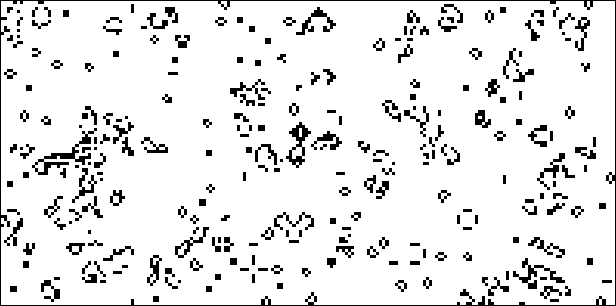
\includegraphics[width=1.0\textwidth]{./images/CA_FDM/game-of-life}
\end{figure}
A famous block for example is the \emph{glider} ( see picture \ref{fig:glider}) that is a 5-step-period pattern that is capable of moving into the cellular space.

\subsubsection{Game of life as Turing machine}
Every CA con be considered a device capable of supporting computation and the
initial configuration can encode an input string (a program for example). At
some point the current configuration can be interpreted as the result of the
computation and decoded in a output string. But as we stated before in section
\ref{DFA} not all the computational device have the same computational power. So
which is the one of the game of life? Life was proved can compute everything a
universal Turing machine can, and under Turing-Church's thesis, everything can
be computed by a computer\cite{berlekamp1982}.
\begin{figure}
\centering
\caption{Glider in Conway's game of life.}
\label{fig:glider}
\setlength{\fboxrule}{1pt}%
\fbox{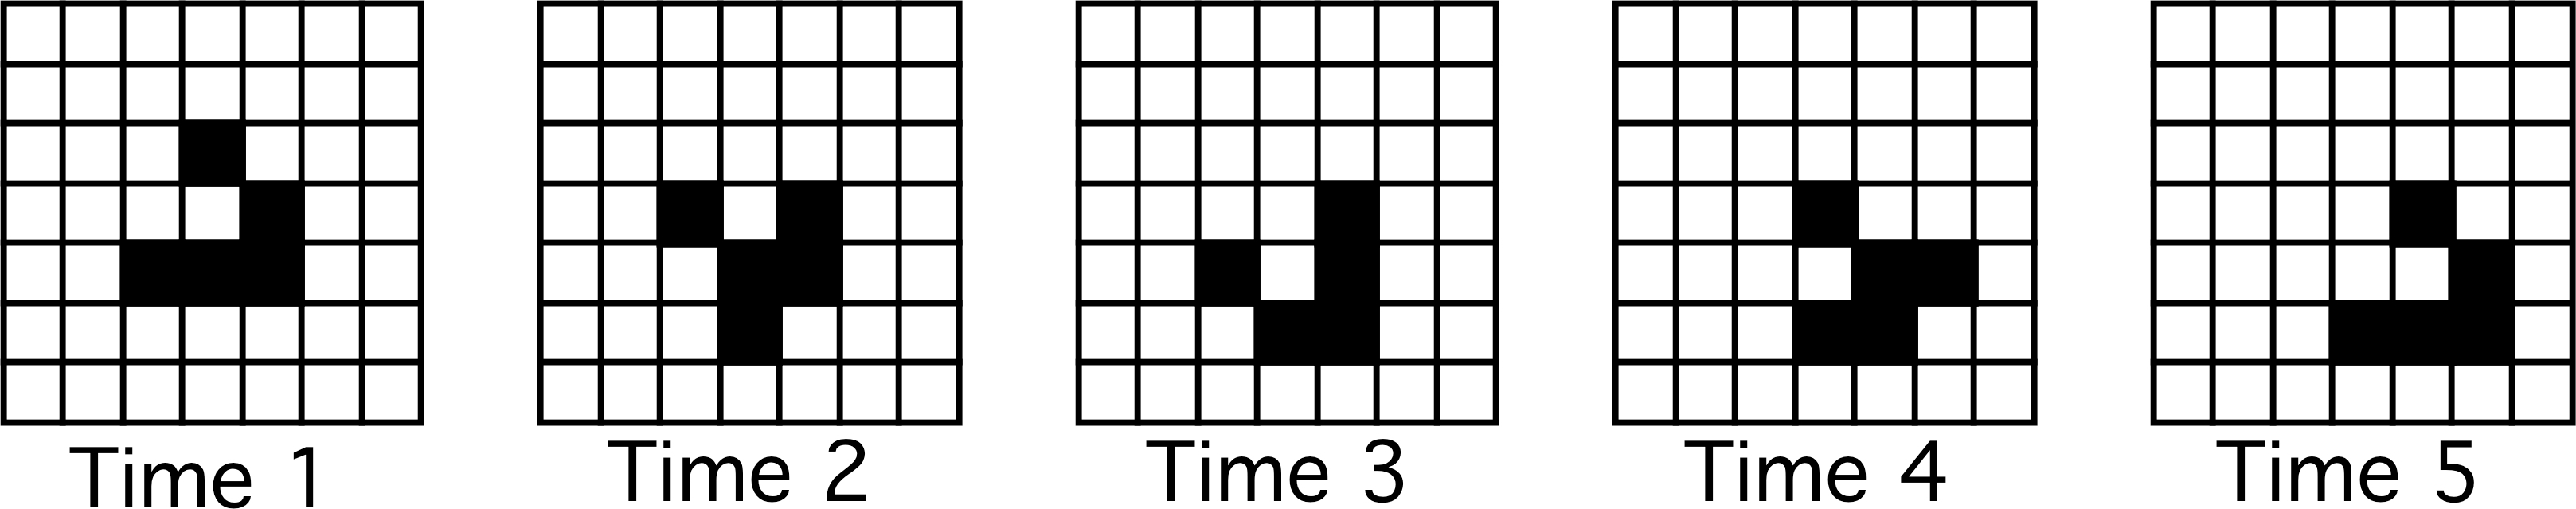
\includegraphics[width=1.0\textwidth]{./images/CA_FDM/glider}}
\end{figure}



This raises a computational issue; given the \emph{Halting
Theorem}\footnote{There can not be any algorithm to decide whether, given an
input, a Turing machine will accept or not.} the evolution of \emph{Life} is
unpredictable (as all the universal computational systems) so it means that is
not possible to use any algorithmically shortcuts to anticipate the resulting
configuration given an initial input. The most efficient way is to let the
system run.

\begin{quotation}
\em Life, like all computationally universal systems, defines the most efficient
simulation of its own behavior\cite{Ilachinski2001}
\end{quotation}





\section{Extension of the Cellular automata model}
It is possible to relax some of the assumptions in the general characterization
of CA provided in the ordinary CA definitions and get interesting results.
Asynchronous updating of the cell, non homogenous lattice with different
neighborhood or transition functions.

\subsection{Probabilistic CA}
Probabilist CA is are an extension of the common CA paradigm. They share all
the basic concept of an ordinary homogeneous
CA with an important difference in the transition function.
\begin{math}\sigma\end{math} is a stochastic-function that choose the next-state
according to some probability distributions. They are used in a wide class of
problems like in modelling ferromagnetism, statistical mechanics
\cite{Vichniac1984} or the cellular Potts model\footnote{Is a computational
lattice-based model to simulate the collective behavior of cellular structures.}


\subsubsection{Cellular automata as Markov process}
Another approach in studying CA, even if it is probably not a practical
way to study the CA is to see CA as a Markov process\footnote{Name for the
Russian mathematician Andrey Markov best known for his work on stochastic
processes.}. A Markov process, is a stochastic process that exhibits
memorylessness \footnote{Also called Markov property.} and it means that the
future state is conditionally independent\footnote{Two event
\begin{math}A\end{math} and \begin{math}B\end{math} are independent if
\begin{math}P(A B)=P(A)P(B)\end{math} or in other words that the conditional
probability \begin{math}P(A|B)=P(A)\end{math}.} of the past.
This property of the process means that future probabilities of an event may be
determined from the probabilities of events at the current time.
More formally if a process has this property following  equation holds:
\begin{align*}
P(X(t_n)&= x \,| X\,(t_1) = x_1,X(t_2) = x_2, \ldots,X(t_{n-1})=x_{n-1}) \\
&= P(X(t_n)=x | X(t_{n-1}=x_{n-1})
\end{align*}

In PCA analysis we are more interested in Markov chain because each cell has a
discrete set of possible value for the status variable.
In terms of chain a CA is a process that starts in one of these states and moves
successively from one state to another. If the chain is currently in state
\begin{math}s_i\end{math}, than it evolve to state \begin{math}s_j\end{math} at
the next step with probability \begin{math}p_{ij}\end{math}.The changes of state
of the system are called transitions, and the probabilities associated with
various state changes are called transition probabilities usually represented
in the Markov chain transition matrix :
\[
M =
\left( {\begin{array}{cccc}
p_{11} & p_{12} & p_{13} &\cdots \\
p_{21} & p_{12} & p_{23} &\cdots \\
p_{31} & p_{32} & p_{33} &\cdots \\
\vdots & \vdots  &\vdots& \ddots\\
\end{array} } \right)
\]

This could seems to be a good way to analyze the probabilistic CA but, a
small grid  \begin{math}10\times10\end{math} (common models model use grid
\begin{math}100\times100\end{math} or larger) identify
\begin{math}2^{10\times10}\end{math}possible states and the resulting matrix
dimension of \begin{math}2^{10\times10}\times2^{10\times10}\end{math} that is a
very large number!


